\documentclass[12pt]{article}
\usepackage[margin=1in]{geometry}
\usepackage{amsmath,amsfonts,amsthm,amssymb}
\usepackage{graphicx} 

\title{Stochastic Recursions Tutorial}

\author{Daniel Selsam}
\date{}
 
\begin{document}

\maketitle


\begin{figure}
\hspace{-0.5in}
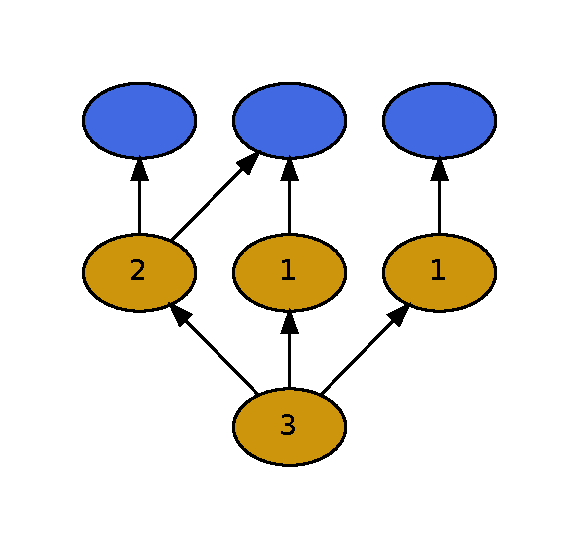
\includegraphics[width=1.5in]{tutorial_1/dot1.pdf}
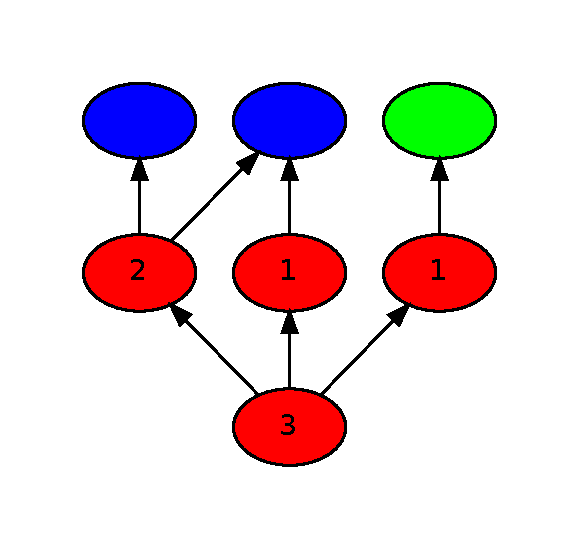
\includegraphics[width=1.5in]{tutorial_1/dot2.pdf}
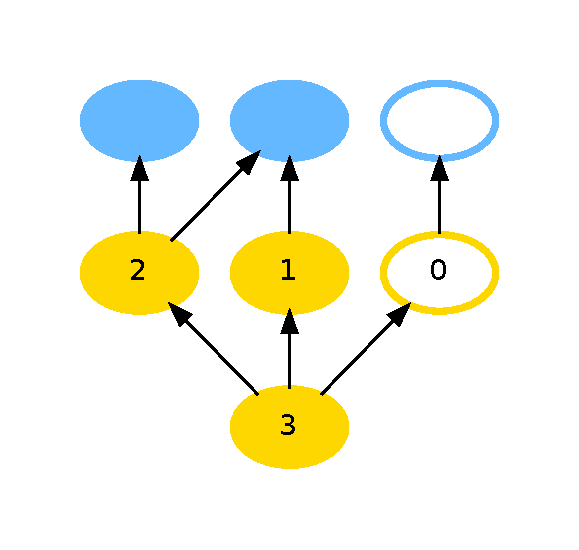
\includegraphics[width=1.5in]{tutorial_1/dot3.pdf}
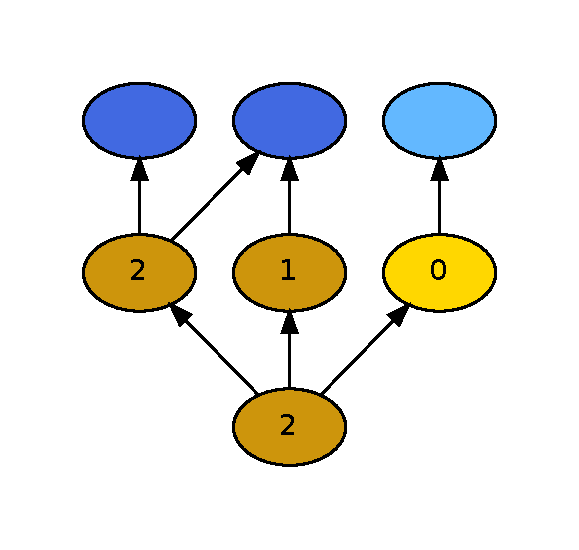
\includegraphics[width=1.5in]{tutorial_1/dot4.pdf}
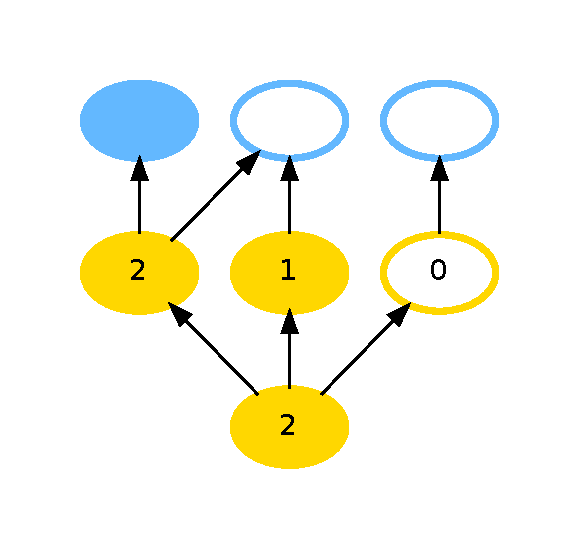
\includegraphics[width=1.5in]{tutorial_1/dot5.pdf}
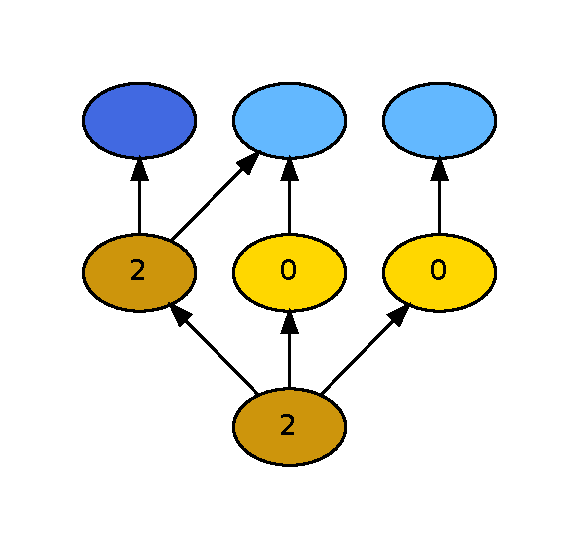
\includegraphics[width=1.5in]{tutorial_1/dot6.pdf}
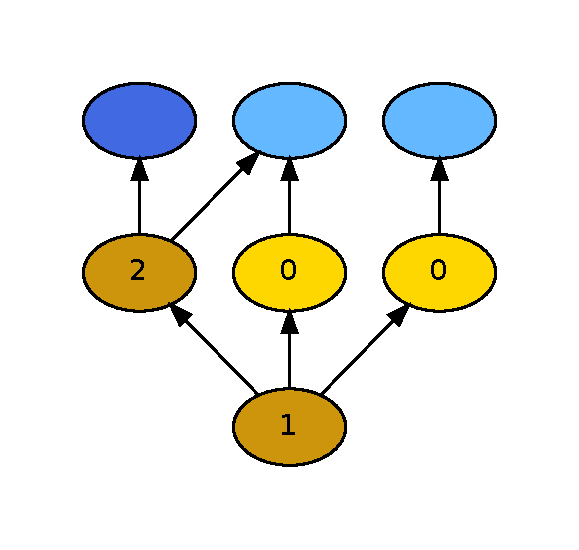
\includegraphics[width=1.5in]{tutorial_1/dot7.pdf}
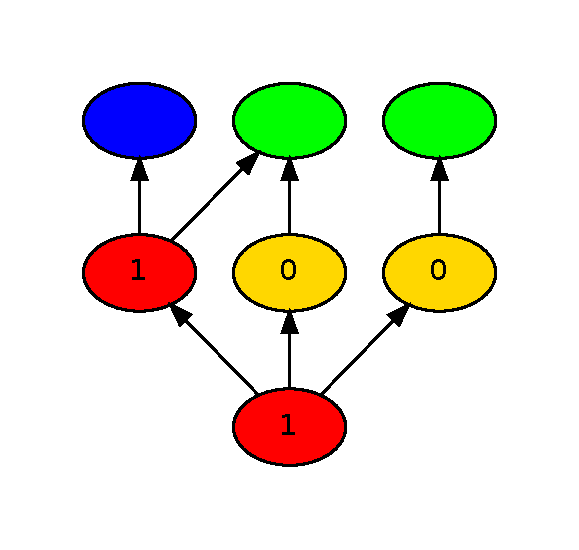
\includegraphics[width=1.5in]{tutorial_1/dot8.pdf}
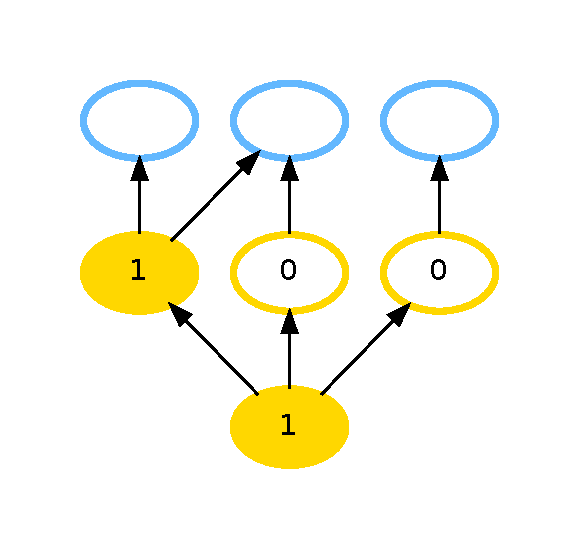
\includegraphics[width=1.5in]{tutorial_1/dot9.pdf}
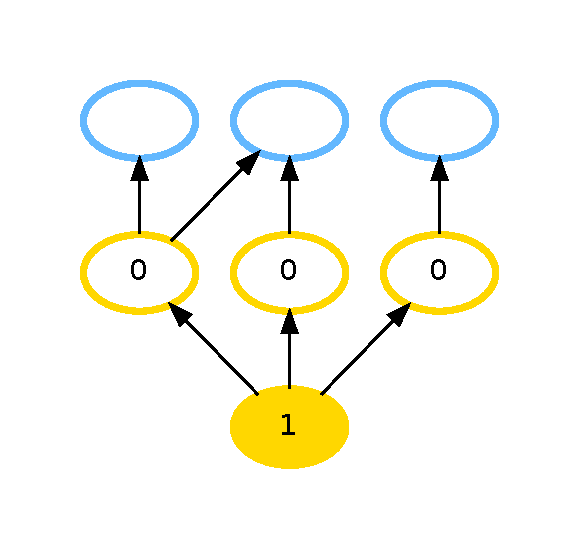
\includegraphics[width=1.5in]{tutorial_1/dot10.pdf}
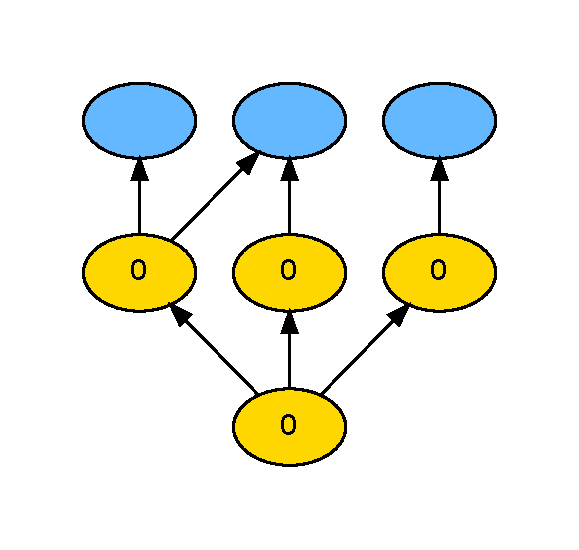
\includegraphics[width=1.5in]{tutorial_1/dot11.pdf}
\caption{Detach}
\label{fig:detach}
\end{figure}

\begin{figure}
\hspace{-0.5in}
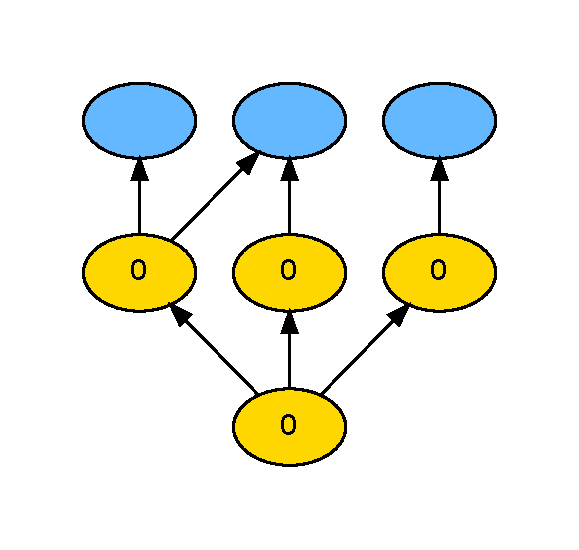
\includegraphics[width=1.5in]{tutorial_1/dot11.pdf}
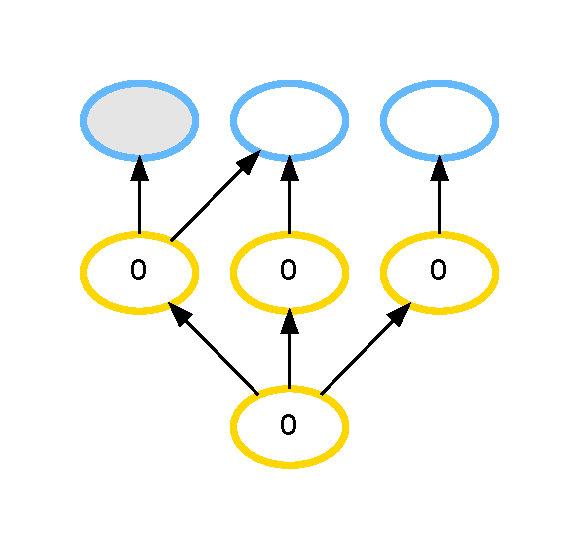
\includegraphics[width=1.5in]{tutorial_1/dot12.pdf}
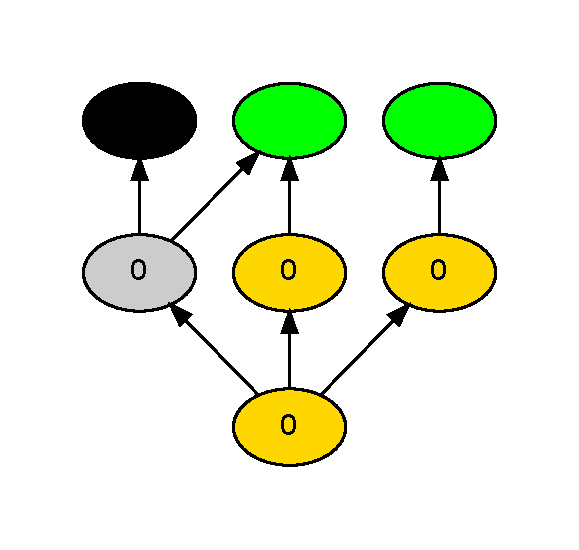
\includegraphics[width=1.5in]{tutorial_1/dot13.pdf}
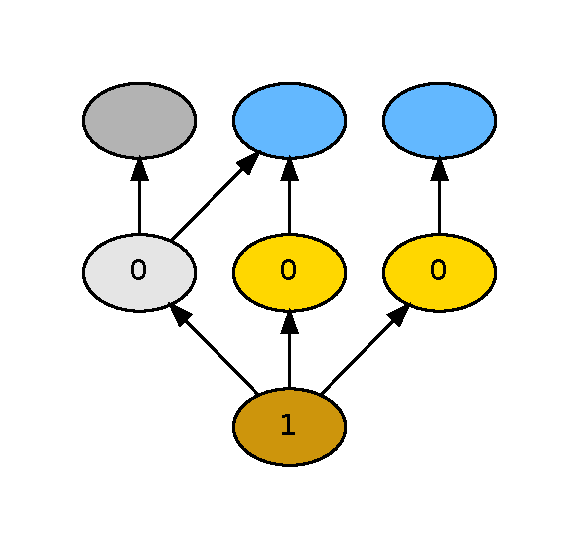
\includegraphics[width=1.5in]{tutorial_1/dot14.pdf}
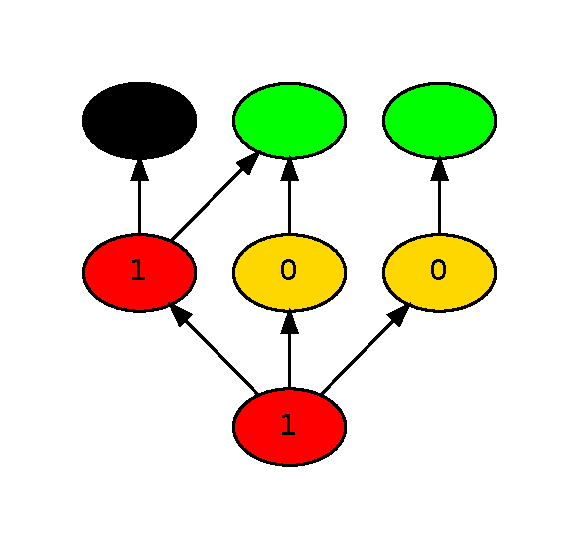
\includegraphics[width=1.5in]{tutorial_1/dot15.pdf}
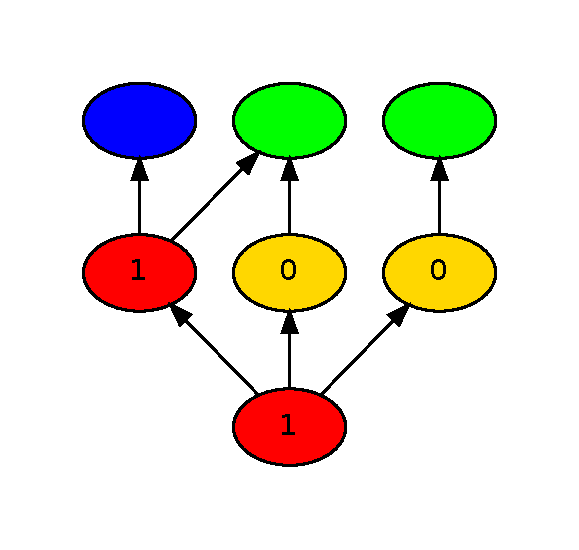
\includegraphics[width=1.5in]{tutorial_1/dot16.pdf}
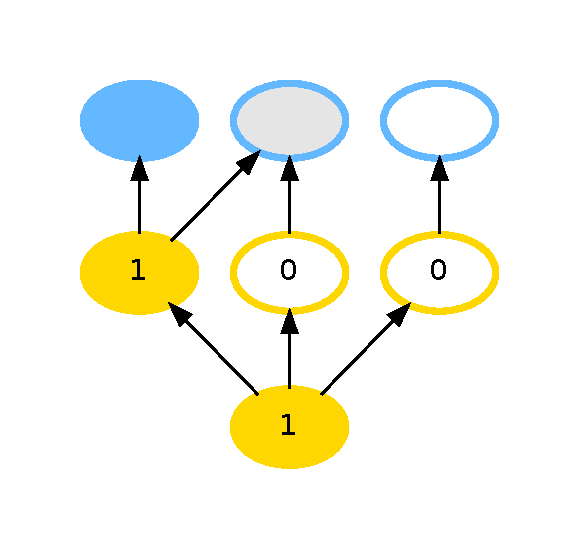
\includegraphics[width=1.5in]{tutorial_1/dot17.pdf}
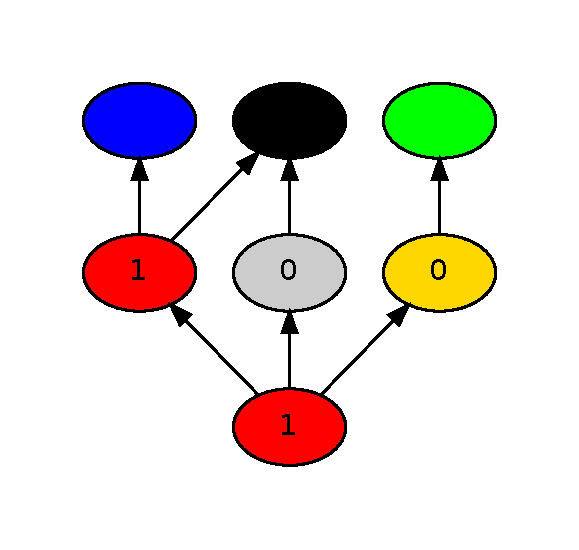
\includegraphics[width=1.5in]{tutorial_1/dot18.pdf}
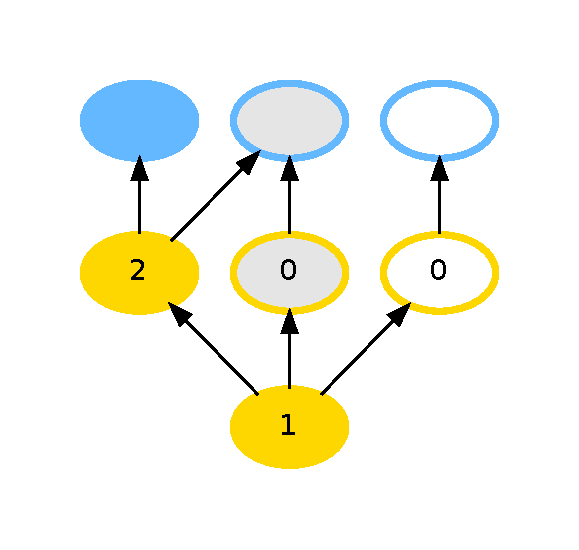
\includegraphics[width=1.5in]{tutorial_1/dot19.pdf}
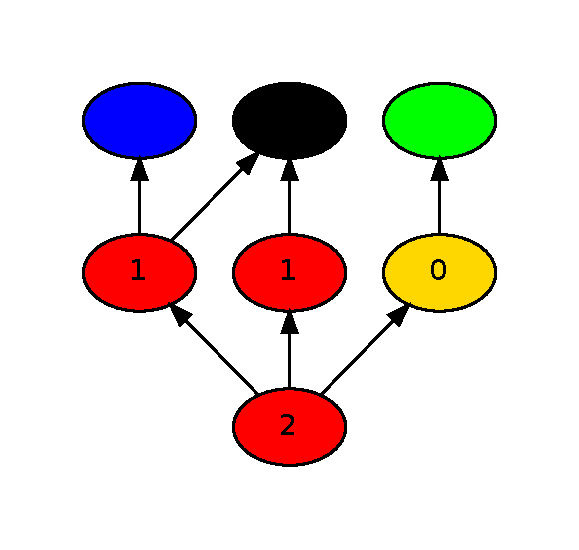
\includegraphics[width=1.5in]{tutorial_1/dot20.pdf}
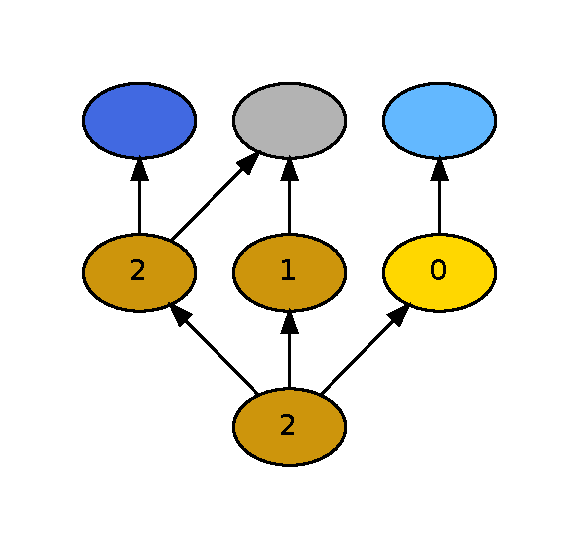
\includegraphics[width=1.5in]{tutorial_1/dot21.pdf}
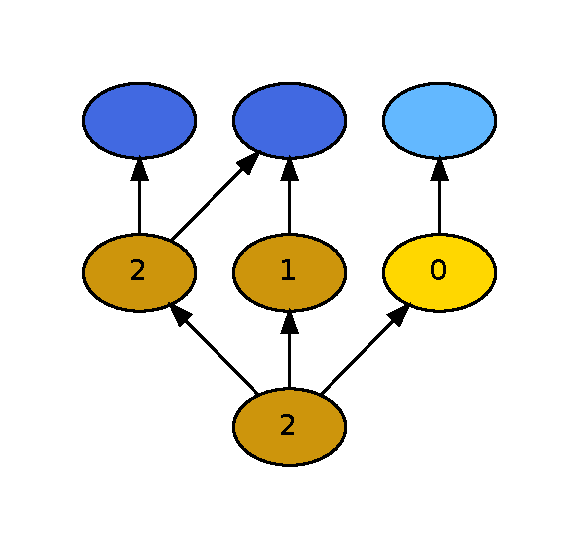
\includegraphics[width=1.5in]{tutorial_1/dot22.pdf}
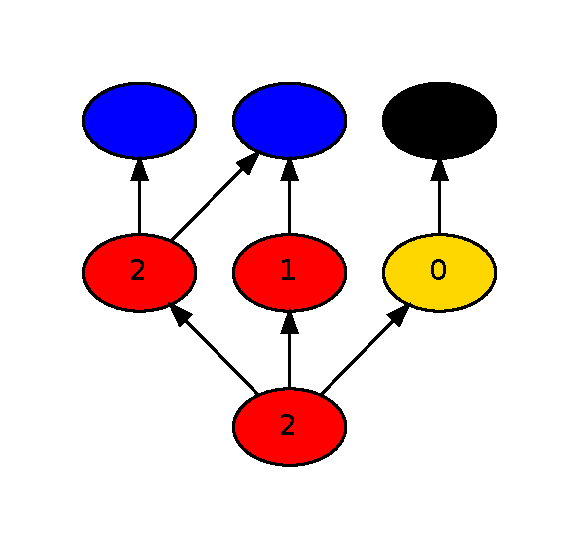
\includegraphics[width=1.5in]{tutorial_1/dot23.pdf}
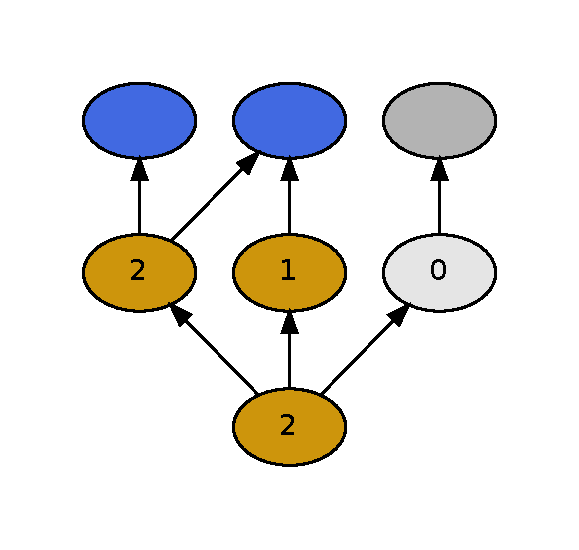
\includegraphics[width=1.5in]{tutorial_1/dot24.pdf}
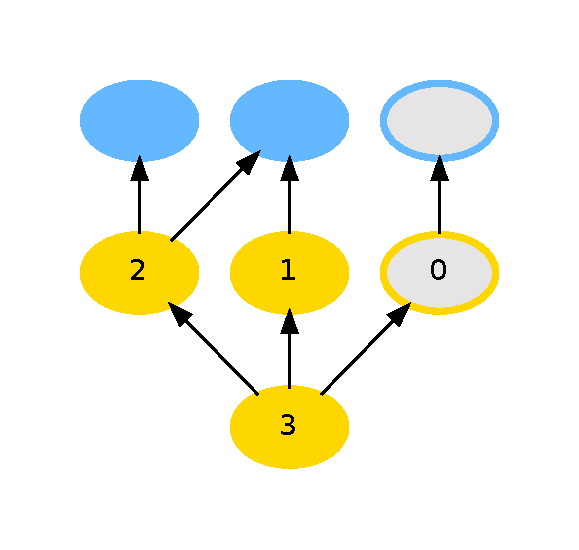
\includegraphics[width=1.5in]{tutorial_1/dot25.pdf}
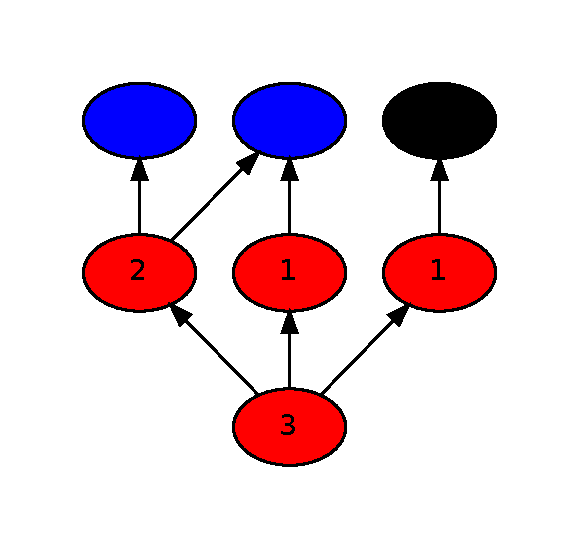
\includegraphics[width=1.5in]{tutorial_1/dot26.pdf}
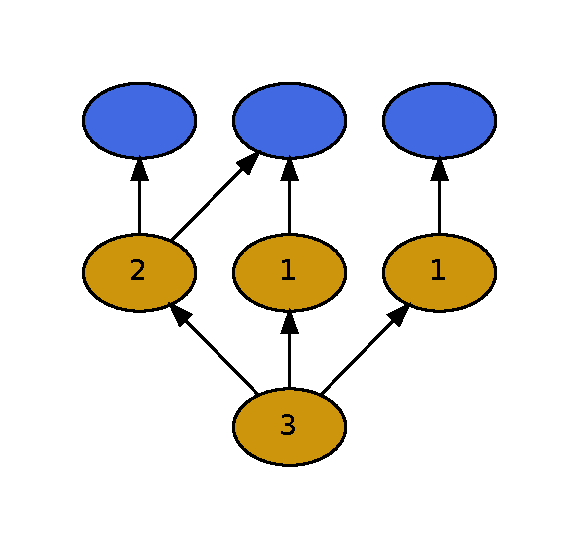
\includegraphics[width=1.5in]{tutorial_1/dot27.pdf}
\caption{Regen}
\label{fig:regen}
\end{figure}



\end{document}
